% LambdaCube-CL.tex
\begin{hcarentry}[updated]{LambdaCube}
\report{Csaba Hruska}%05/12
\status{experimental, active development}
\makeheader

LambdaCube is a 3D graphics library entirely written in Haskell.

The main goal of this project is to provide a modern and feature rich
graphical backend for various Haskell projects, and in the long run it
is intended to be a practical solution even for serious purposes.
With LambdaCube we can program the GPU in a purely functional manner,
just like with GPipe, but LambdaCube provides much better runtime
performance.

Over the last few months, the library has been completely rewritten.
The current API is a rudimentary EDSL that is not intended for direct
use in the long run.  It is essentially the internal phase of a
compiler backend exposed for testing purposes.  To exercise the library, we
have created two small proof of concept examples: a port of the old
LambdaCube Stunts example, and a Quake III level viewer.

Our mid term plan is to define a standalone DSL, so the graphics
pipeline could be dynamically reprogrammed during runtime.  Using our
graphics language, we can implement arbitrary rendering techniques in
a hardware independent and compositional way.  All resource handling
and performance optimizations will be done by the graphics backend.
Currently we are targeting OpenGL 3.3, but OpenGL ES support is
also planned.

Everyone is invited to contribute! You can help the project by playing
around with the code, thinking about API design, finding bugs (well,
there are a lot of them anyway), creating more content to display, and
generally stress testing the library as much as possible by using it
in your own projects.

%**<img width=500 src="./lc-q3.png">
%*ignore
\begin{center}
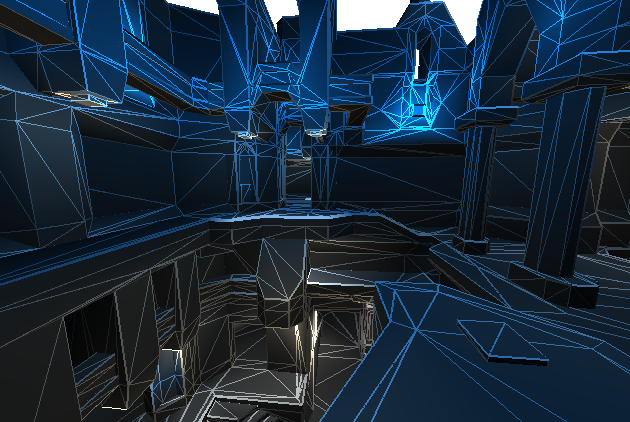
\includegraphics[width=0.47\textwidth]{html/lc-q3.png}
\end{center}
%*endignore

\FurtherReading
\begin{compactitem}
\item \url{https://github.com/csabahruska/lc-dsl}
\item \url{http://www.haskell.org/haskellwiki/LambdaCubeEngine}
\item \url{http://hackage.haskell.org/package/stunts}
\item \url{http://www.youtube.com/watch?v=kDu5aCGc8l4}
\end{compactitem}
\end{hcarentry}
